%!TeX  root  =  user_guide.tex

\chapter{Использование модулей ядра QGIS}\label{sec:core_plugins}\index{plugins!core}

% когда переработка раздела будет завершена,
% раскоментируйте следующую строку:
%\updatedisclaimer

{\setlength{\extrarowheight}{15pt}
\small
\begin{longtable}{|p{1.2cm}|p{3.8cm}|p{10.5cm}|}
\caption{22 модуля ядра QGIS }\label{tab:core_plugins} \\
\hline
 \textbf{Иконка} & \textbf{Модуль} & \textbf{Описание}\\
\endfirsthead
\hline
\textbf{Иконка} & \textbf{Модуль} & \textbf{Описание}\\
\endhead
\hline

\includegraphics[width=0.6cm]{delimited_text}
 & Текст с разделителями \index{plugins!delimited text} & Загружает и отображает текстовые файлы, содержащие координаты x,y\\
\hline

\includegraphics[width=0.6cm]{coordinate_capture}
 & Захват координат \index{plugins!coordinate capture}& Захват кординат курсора в различных системах координат\\
\hline
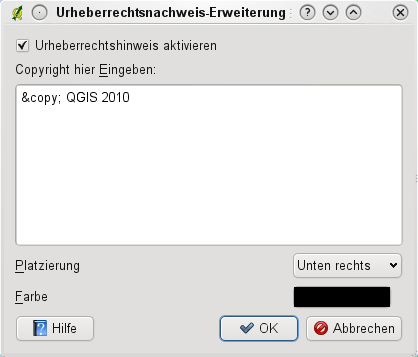
\includegraphics[width=0.6cm]{copyright_label}
 & Знак авторского права \index{plugins!copyright}& Отображает на карте знак авторского права\\
\hline

\includegraphics[width=0.6cm]{diagram_overlay}
 & Наложение диаграмм \index{plugins!diagram}& Размещает диаграмму (круговую или гистограмму) или пропорциональные символы на векторном слое\\
\hline

\includegraphics[width=0.6cm]{dxf2shp_converter}
 & Преобразователь DXF2Shape \index{plugins!DXF2Shape}& Преобразователь файлов из формата DXF в формат SHP\\
\hline
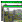
\includegraphics[width=0.6cm]{evis_icon}
 & eVis & Инструмент визуализации события \\
\hline

\includegraphics[width=0.6cm, height=0.6cm]{ftoolslogo}
 & fTools \index{plugins!ftools}& Набор инструментов для анализа, в том числе геометрического, обработке гео-данных и исследований \\
\hline
% 
\includegraphics[width=0.6cm, height=0.6cm]{ftoolslogo}
 & Инструменты GDAL \index{plugins!gdaltools} & Растровые инструменты: упрощенный графический интерфейс для обычно используемых программ\\
\hline

\includegraphics[width=0.6cm]{gps_importer}
 & Инструмент GPS \index{plugins!gps}& Инструмент для загрузки и импорта данных GPS\\
\hline

\includegraphics[width=0.6cm]{grass}
 & GRASS \index{plugin!grass toolbox} & Активация панели инструментов GRASS\\
\hline
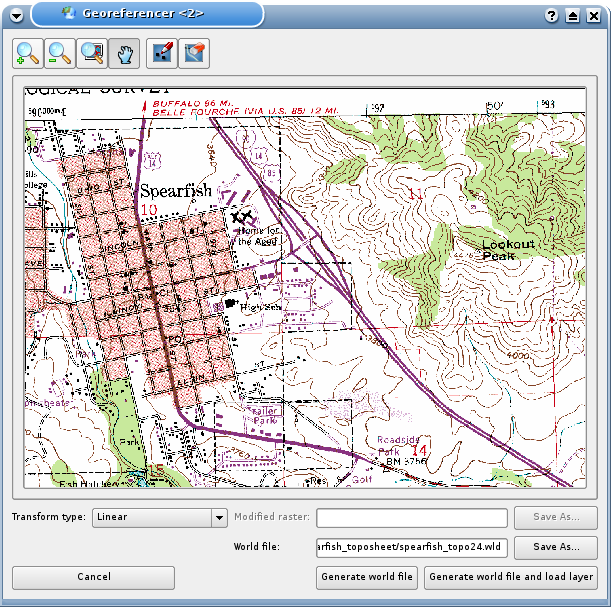
\includegraphics[width=0.6cm]{georeferencer}
 & Гео-привязка растров GDAL \index{plugin!georeferencer} & Гео-привязка растровых данных с использованием GDAL\\
\hline

\includegraphics[width=0.6cm]{interpolation}
& Модуль интерполяции \index{plugins!Interpolation}& Интерполяция по вершинам в векторном слое\\
\hline

\includegraphics[width=0.6cm]{raster_terrain}
& Растровая модель ландшафта \index{plugins!Raster Terrain Modelling}& Расчет наклона, аспекта,
неровностей и общего искривления с использованием цифровых моделей\\
\hline

\includegraphics[width=0.6cm]{mapserver_export}
& Модуль экспорта MapServer \index{plugins!MapServer Export}& Экспорт файла данных проекта QGIS в формат данных MapServer \\
\hline
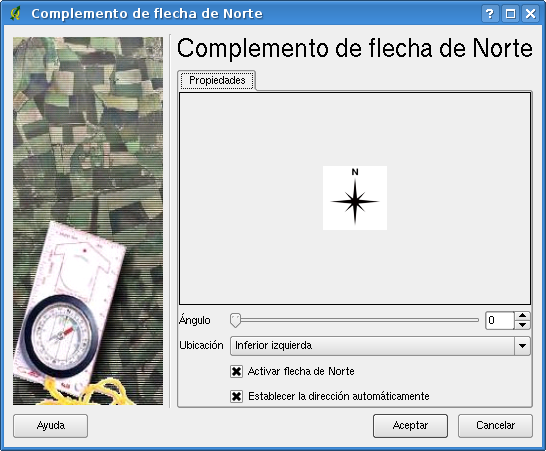
\includegraphics[width=0.6cm]{north_arrow}
& Указатель «Север-Юг» \index{plugins!north arrow}& Вывод на карте указателя <<Север-Юг>>\\
\hline

\includegraphics[width=0.6cm]{ogr_converter}
 & Конвертер слоя OGR \index{plugins!OGR converter} & Конвертация векторных слоёв между поддерживаемыми форматами  OGR\\
\hline
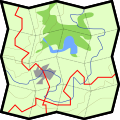
\includegraphics[width=0.6cm]{osm_icon}
 & OpenStreetMap & Отображение и редактирование данных  OpenStreetMap\\
\hline

\includegraphics[width=0.6cm]{oracle_raster}
 & Oracle Georaster \index{plugins!georaster}& Доступ к данным  Oracle Spatial GeoRasters\\
\hline

\includegraphics[width=0.6cm]{plugin_installer}
 & Установка модулей \index{plugins!Plugin Installer} & Загрузка и установка модулей QGIS на языке Python\\
\hline

\includegraphics[width=0.6cm]{spiticon}
 & SPIT \index{plugins!spit}& Инструмент импорта shp-файлов в  PostgreSQL/PostGIS\\
\hline

\includegraphics[width=0.6cm]{quick_print}
 & Быстрая печать \index{plugins!quick print}& Быстрая печать карты с минимальными усилиями\\
\hline
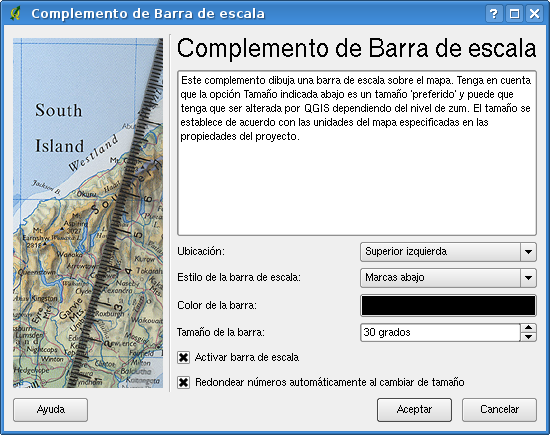
\includegraphics[width=0.6cm]{scale_bar}
 & Масштабная линейка \index{plugins!scalebar}& Отображает на карте масштабную линейку\\
\hline

\includegraphics[width=0.6cm]{mIconAddWfsLayer}
 & WFS & Загружает и отображает слои WFS\\
\hline
\end{longtable}}
